\documentclass[tikz,border=8pt]{standalone}
% Shared look for every TikZ diagram. Load with \input{../../tools/tikz-style.tex}
\usepackage[T1]{fontenc}
\usepackage{lmodern}
\renewcommand{\sfdefault}{lmr}  % diagrams use the same serif as the text
\usetikzlibrary{arrows.meta, positioning, shapes.geometric, calc, fit, backgrounds}
\definecolor{cblue}{HTML}{4C78A8}
\definecolor{corange}{HTML}{F58518}
\definecolor{cgreen}{HTML}{54A24B}
\definecolor{cred}{HTML}{E45756}
\definecolor{cpurple}{HTML}{B279A2}
\definecolor{cgrey}{HTML}{6B6B6B}
\tikzset{
  every picture/.style={font=\sffamily, line width=1.2pt},
  box/.style={draw=#1, fill=#1!12, rounded corners=4pt, align=center, inner sep=7pt, minimum height=1.1cm},
  box/.default=cgrey,
  arrow/.style={-{Stealth[length=3mm]}, draw=cgrey, line width=1.4pt},
  title/.style={font=\sffamily\bfseries\Large},
  note/.style={font=\sffamily\small, text=cgrey, align=center},
}
\AtBeginDocument{\hyphenpenalty=10000 \exhyphenpenalty=10000}

\usepackage{colortbl}
\begin{document}
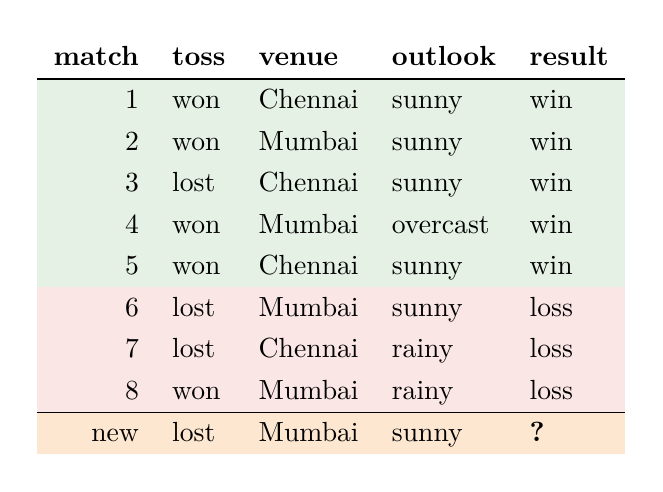
\begin{tikzpicture}
  \node {\renewcommand{\arraystretch}{1.25}%
  \begin{tabular}{rllll}
    \textbf{match} & \textbf{toss} & \textbf{venue} & \textbf{outlook} & \textbf{result} \\ \hline
    \rowcolor{cgreen!15} 1 & won & Chennai & sunny & win \\
    \rowcolor{cgreen!15} 2 & won & Mumbai & sunny & win \\
    \rowcolor{cgreen!15} 3 & lost & Chennai & sunny & win \\
    \rowcolor{cgreen!15} 4 & won & Mumbai & overcast & win \\
    \rowcolor{cgreen!15} 5 & won & Chennai & sunny & win \\
    \rowcolor{cred!15} 6 & lost & Mumbai & sunny & loss \\
    \rowcolor{cred!15} 7 & lost & Chennai & rainy & loss \\
    \rowcolor{cred!15} 8 & won & Mumbai & rainy & loss \\ \hline
    \rowcolor{corange!20} new & lost & Mumbai & sunny & \textbf{?} \\
  \end{tabular}};
\end{tikzpicture}
\end{document}
